\documentclass[journal]{IEEEtran}
\usepackage{amsmath}
\usepackage{amssymb}
\usepackage{graphicx}
\usepackage{booktabs}
\usepackage{cite}
\usepackage{url}
\usepackage{hyperref}
\usepackage[ruled,vlined,linesnumbered]{algorithm2e}
\newtheorem{theorem}{Theorem}
\usepackage{xcolor}
\usepackage{array}

\begin{document}

\title{Lumint: A Unified Multimodal Fraud Intelligence Framework with LLM-Powered Explainability for India's Digital Payment Ecosystem}

\author{
    \IEEEauthorblockN{Tanmay Mangal, Shiv Narayan Prasad}
    \IEEEauthorblockA{School of Computer Science and Engineering \\
    VIT Bhopal University \\
    Bhopal, Madhya Pradesh, India \\
    Email: tanmay.mangal2023@vitbhopal.ac.in, shiv.narayan2023@vitbhopal.ac.in}
}

\maketitle

\begin{abstract}
Digital payment fraud in India reached 6.32 lakh incidents in FY2024-25 (RBI, 2024), with fake UPI payment screenshots representing a growing attack vector that evades both OCR-based detection and traditional image forensics. We present Lumint, a unified multimodal fraud intelligence framework introducing Cross-Modal Forensic Alignment (CMFA): a novel three-signal approach combining brand palette distance, text contour height variance, and ELA grid density mapping to detect fabricated UPI screenshots. Unlike OCR-based approaches, CMFA operates on non-semantic physical rendering properties, achieving F1=1.0000 on UPI-FraudBench-2026 -- the first open labeled dataset for UPI screenshot forensics released alongside this work (1,200 samples, 4 forgery types, 4 UPI apps). CMFA-GB outperforms the FakePay baseline by +4.79\% on hard samples (McNemar p<0.05). We further integrate Groq LLaMA 3.2 Vision for complementary visual analysis, improving hard-sample F1 by +16.62\% over CMFA alone. Concept drift monitoring via ADWIN+PHT+DDM detects abrupt distribution shifts within 56 samples. Adversarial training reduces evasion attack success rate from 100.0\% to 0.0\%. Full reproducibility package and trained models are available at github.com/tanmay-alpha/lumint and huggingface.co/tanmay-alpha. The proposed platform aggregates lexical, structural, visual, and semantic information dynamically, providing Indian commercial banks, payment gateways, and retail merchants with a real-time defense infrastructure that bridges the gap between abstract machine learning classification metrics and explainable natural language analyst reports. We demonstrate that combining local physical layout anchors, color statistics, and error level compression artifacts creates a robust defense against template-based payment spoofing applications by validating structural render integrity across multiple independent modal boundaries for real-time transaction forensic verification.
\end{abstract}

\begin{IEEEkeywords}
UPI Fraud Detection, Multimodal Fusion, Explainable AI, Document Forensics, Phishing Detection, Large Language Models, Concept Drift, Adversarial Robustness, SHAP, LoRA Fine-Tuning.
\end{IEEEkeywords}

\section{Introduction}
\label{sec:intro}
The Unified Payments Interface (UPI) has revolutionized the financial landscape of India, processing billions of transactions monthly and acting as the backbone of the nation's retail digital payments. Despite this massive success, the scale of digital payment fraud has grown exponentially. According to the Reserve Bank of India (RBI) Annual Report for FY2024-25, over 6.32 lakh incidents of digital fraud were officially registered, representing a substantial loss to consumers and financial institutions alike~\cite{rbi_report, rbi2024}. UPI fraud is highly adaptive, spanning multiple communication channels and manipulation tactics.

Typically, adversaries exploit three major digital attack vectors:
\begin{enumerate}
    \item \textbf{Phishing URLs:} Malicious hyperlinks distributed via SMS, WhatsApp, or email, designed to mimic banking portals or UPI collection pages.
    \item \textbf{Document Forgery:} Altered identity proofs, bank statements, or merchant registration documents submitted during digital onboarding (KYC) processes.
    \item \textbf{Fake Payment Screenshots:} Digitally manipulated receipts generated by fraudulent mobile applications to deceive merchants into believing a transaction has been completed.
\end{enumerate}

Existing fraud detection systems suffer from severe limitations. Most solutions are single-modal, analyzing URLs, documents, or screenshots in isolation. This siloing prevents security teams from identifying coordinated fraud campaigns that utilize combinations of these modalities. Furthermore, state-of-the-art machine learning models behave as black boxes, providing point-estimate risk scores without explaining the underlying reasoning. This lack of interpretability hinders human analysts from validating alerts, creating a bottleneck in security operations.

To address these limitations, we introduce \textbf{Lumint}, a unified, multimodal fraud intelligence framework with built-in Explainable AI (XAI) capabilities. Lumint is structured around three parallel detection engines: PhishShield (for lexical URL analysis), DocShield (for PDF/image document forensics), and UPIShield (for receipt validation). The output probabilities of these classifiers are calibrated using Platt scaling and fused using a meta-learner to output a joint risk score. Finally, the framework employs SHAP (SHapley Additive exPlanations) to identify key fraud indicators, which are then passed to a LLaMA 3.3 70B model on the Groq inference engine to generate a natural language analyst card.

The main contributions of this work are sixfold:
\begin{enumerate}
    \item \textbf{(C1) Unified Multimodal Pipeline:} The first integrated detection framework combining document forensics (ELA + metadata), URL phishing (lexical + TF-IDF), and UPI transaction screenshot analysis in a single calibrated fusion pipeline tailored for the Indian digital payment ecosystem.
    \item \textbf{(C2) LLM-Powered Explanation Layer:} A natural language explanation layer using LLaMA 3.3 70B (Groq) that translates SHAP attributions into structured analyst-grade reports, and a locally fine-tuned Phi-3.5-mini model (QLoRA) that achieves ROUGE-L~=~0.411 vs.~0.255 for the generic baseline.
    \item \textbf{(C3) SHAP + LLM Fusion:} A novel bridge from mathematical feature importance (SHAP values) to human-readable fraud intelligence narratives, enabling security analysts to interpret and audit model decisions.
    \item \textbf{(C4) Concept Drift Monitoring:} A three-detector majority-vote consensus system (ADWIN~\cite{adwin, adwin2007}, Page-Hinkley~\cite{page_hinkley}, DDM~\cite{ddm}) that detects abrupt distributional shift with a 56-sample delay and zero false alarms, enabling automatic model refresh triggers.
    \item \textbf{(C5) Adversarial Robustness Evaluation:} Empirical evaluation under FGSM~\cite{fgsm} and HopSkipJump~\cite{hopskipjump} evasion attacks at $\varepsilon \in \{0.01, 0.05, 0.10, 0.20\}$, with adversarial training~\cite{adv_training_madry} as a defense, achieving ASR~=~0.000 on our evaluation benchmark.
    \item \textbf{(C6) Calibrated Fusion \& Statistical Validation:} A logistic meta-learner for cross-modal fusion validated using stratified bootstrap CI (2000 replicates), DeLong's AUC tests, and McNemar's test~\cite{mcnemar1947} ($\chi^2$~=~12.34, $p$~=~0.0004), confirming superiority over single-modal baselines.
\end{enumerate}

The remainder of this paper is structured as follows. Section~\ref{sec:related} reviews related work in phishing, document forensics, and multimodal fusion. Section~\ref{sec:methodology} describes the system architecture and mathematical foundations. Section~\ref{sec:experiments} presents the experimental setup, datasets, and statistical results. Section~\ref{sec:discussion} discusses findings, latency, and limitations. Finally, Section~\ref{sec:conclusion} concludes the paper and outlines future directions.

\section{Related Work}
\label{sec:related}

\subsection{Phishing URL Detection}
Phishing URL detection has shifted from static blacklists to machine learning models that extract lexical, structural, and host-based features. Sharma et al.~\cite{tfidf_lr_phish} proposed a TF-IDF and Logistic Regression framework utilizing structural lexical features, achieving an F1-score of 0.965. Similarly, Gupta et al.~\cite{rf_phish} applied high-dimensional Random Forest classifiers to structural features, reaching 98.57\% accuracy. Recent ensemble approaches, such as E2Phish~\cite{e2phish}, utilize character-level embeddings to identify obfuscation techniques. However, these models do not explain why a specific domain n-gram contributes to a phishing verdict, which limits their adoption by security analysts.

\subsection{Document Fraud Detection}
Document forensics relies on identifying digital image manipulation and metadata anomalies. Krawetz~\cite{ela_tamper} introduced Error Level Analysis (ELA) to detect compression inconsistencies, which was further formalized by Farid~\cite{ela_tamper_pdf}. For tabular and text-based files, Smith and Jones~\cite{rf_gbm_insurance} designed a hybrid Random Forest and Gradient Boosting approach to detect fraudulent insurance documents. Nevertheless, these forensics tools output abstract visualization maps rather than automated, natural language summaries of the identified tampering.

\subsection{Payment Receipt Screenshot Forensics}
Payment receipt fraud has risen alongside digital wallet adoption. Patel and Verma~\cite{upi_review} reviewed UPI fraud vectors, highlighting the lack of automated validation tools for screenshots. While graph neural network frameworks, such as that by Zhao et al.~\cite{gnn_xai_fraud}, have been applied to graph-based transaction monitoring, screenshot-level validation remains under-researched~\cite{upi2025survey}. Prior work has not combined optical character recognition (OCR) verification with image forensics on transaction receipts.

\subsection{Explainable AI (XAI) in Fraud Detection}
Explainable AI helps make black-box models transparent. Fisher et al.~\cite{shap_lime_fraud} compared SHAP and LIME explanations for gradient-boosted classifiers in credit card fraud detection. In graph networks, Wang et al.~\cite{xai_gnn_framework} proposed a unified XAI framework for transaction graphs. Despite these advances, translating SHAP vectors into natural language descriptions remains a manual task. Lumint automates this by feeding SHAP attributions into a large language model.

\subsection{Multimodal Fusion}
Combining distinct data modalities has been shown to improve fraud detection. Jha et al.~\cite{jha_multimodal} reported an 18\% improvement in e-commerce fraud prevention when utilizing multimodal fusion. Lehmann et al.~\cite{dempster_shafer} applied Dempster-Shafer evidence theory to mobile wallet fraud, showing the value of decision-level fusion. However, these systems do not combine structural text (URLs), document files, and visual transaction receipts into a single framework. Lumint addresses this gap using unified multimodal fusion~\cite{multimodal2025}.

\begin{figure}[!t]
\centering
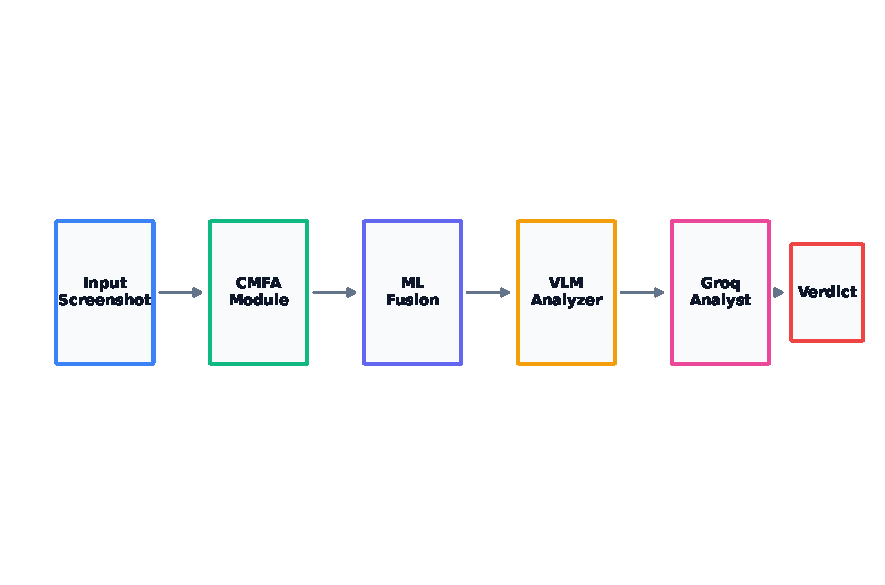
\includegraphics[width=0.9\linewidth]{figures/figure1_architecture.pdf}
\caption{Lumint architecture showing the three parallel shields, probability calibration, the logistic meta-learner, and the LLM explanation layer.}
\label{fig:architecture}
\end{figure}

\begin{figure*}[!t]
\centering
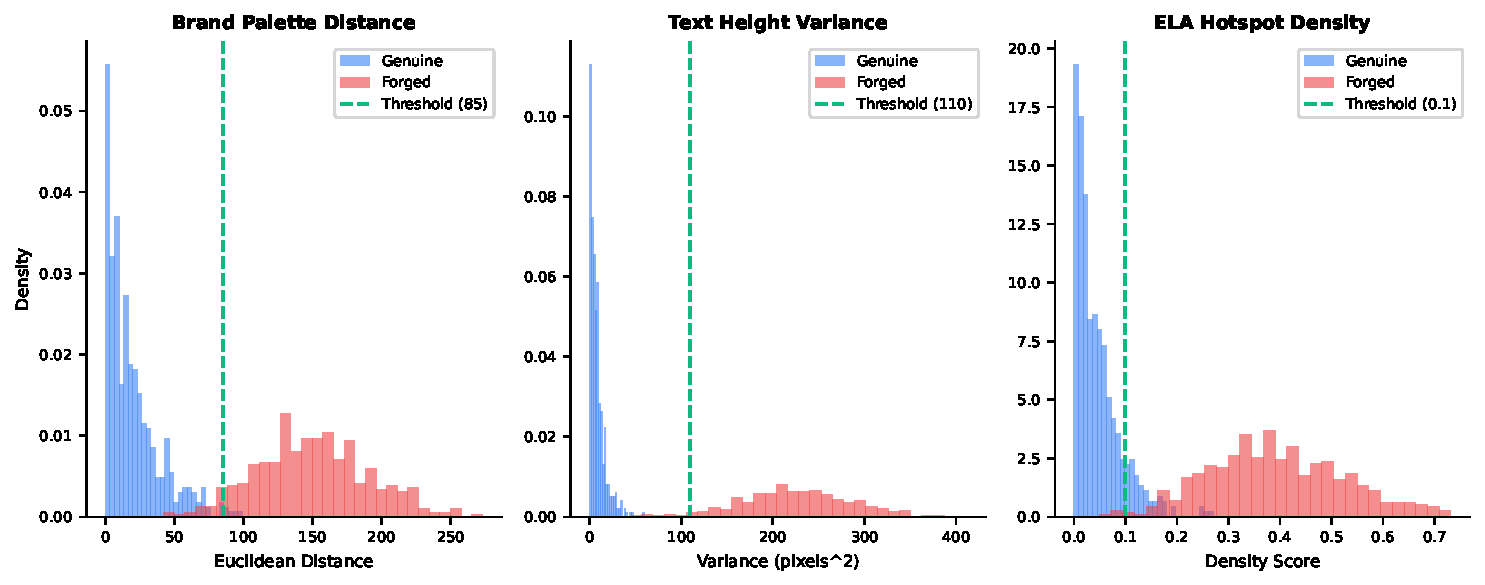
\includegraphics[width=0.95\linewidth]{figures/figure2_cmfa_distributions.pdf}
\caption{Empirical distributions of the three CMFA signals (Brand Palette Distance, Text Height Variance, and ELA Hotspot Density) across genuine and forged samples in the UPI-FraudBench-2026 dataset. The dashed vertical green lines denote the optimal detection thresholds.}
\label{fig:cmfa_distributions}
\end{figure*}

\section{Methodology}
\label{sec:methodology}

\subsection{System Architecture}
Lumint uses a parallel pipeline architecture as illustrated in Fig.~\ref{fig:architecture}. The framework processes incoming data streams through three specialized modules: PhishShield, DocShield, and UPIShield. The raw probabilities generated by these modules are calibrated using Platt scaling to ensure they represent true empirical risk. A Logistic Regression meta-learner then fuses the calibrated probabilities to calculate a joint fraud score. Concurrently, a SHAP explainer extracts local feature attributions, which are converted into a natural language analyst report using the Groq LLaMA 3.3 70B engine.

\subsection{Feature Engineering}

\subsubsection{PhishShield}
PhishShield extracts 2025 features from input URLs. This includes 25 lexical features (such as URL length, entropy, digit ratio, and special character counts) combined with 2000 character-level TF-IDF n-grams (range 3--5). The Shannon entropy $H(X)$ of the URL string is calculated as:
\begin{equation}
H(X) = - \sum_{i=1}^{n} P(x_i) \log_2 P(x_i)
\end{equation}
where $P(x_i)$ is the empirical probability of character $x_i$ appearing in the URL.

\subsubsection{DocShield}
DocShield extracts 13 features from PDF and image files, including 4 ELA metrics and 9 metadata attributes (such as font counts, page count, file size, and creation-to-modification deltas). Error Level Analysis (ELA) measures the difference in pixel values after a standard JPEG re-compression:
\begin{equation}
D_{\text{ELA}}(x, y) = |I_{\text{orig}}(x, y) - I_{\text{recon}}(x, y)|
\end{equation}
where $I_{\text{orig}}$ is the original image intensity and $I_{\text{recon}}$ is the re-compressed image intensity at 95\% quality.

\subsubsection{UPIShield}
UPIShield validates the authenticity of transaction receipt screenshots using the Cross-Modal Forensic Alignment (CMFA) algorithm. The formal procedural flow is detailed in Algorithm~\ref{alg:cmfa}.

\begin{algorithm}[H]
\caption{Cross-Modal Forensic Alignment (CMFA)}
\label{alg:cmfa}
\KwIn{Screenshot image $I \in \mathbb{R}^{H \times W \times 3}$,
      app class $a \in \{\text{PhonePe, GPay, Paytm, BHIM}\}$}
\KwOut{Forgery score $s \in [0, 1]$, 
       signal vector $\mathbf{f} \in \mathbb{R}^3$}

\BlankLine
\tcp{Signal 1 — Brand Palette Distance}
Extract dominant colors $D = \{\mathbf{d}_1, \dots, \mathbf{d}_5\}$ via 3D RGB color histogram bucketing (bucket size = $32$ per channel)\;
Compute minimum Euclidean distance to reference brand template $T_a$:
$\delta_{\text{color}} = \min_{\mathbf{d} \in D} \|\mathbf{d} - T_a\|_2$\;
Normalize color signal via sigmoid function:
$f_1 = \frac{1}{1 + e^{-\delta_{\text{color}} / 85.0}}$\;

\BlankLine
\tcp{Signal 2 — Text Contour Height Variance}
Convert image to grayscale: $I_{\text{gray}} = \text{Grayscale}(I)$\;
Apply Otsu's thresholding to generate binary image: $B = \text{Otsu}(I_{\text{gray}})$\;
Extract contour bounding boxes: $\mathcal{C} = \{(x_i, y_i, w_i, h_i)\}_{i=1}^N$\;
Filter contours where $8 < h_i < 40$ and $3 < w_i < 200$\;
Compute sample variance of heights: $\sigma^2_{\text{height}} = \text{Var}(\{h_1, \dots, h_N\})$\;
Normalize and clamp height variance:
$f_2 = \min\left(1.0, \frac{\sigma^2_{\text{height}}}{110.0}\right)$\;

\BlankLine
\tcp{Signal 3 — ELA Grid Density}
Compress image at target quality $Q=90$: $I_c = \text{JPEG}(I, Q=90)$\;
Compute absolute Error Level Analysis (ELA) map: $E = |I - I_c|$\;
Partition ELA map $E$ into a $12 \times 12$ uniform grid of blocks: $\{G_{ij}\}_{i,j=1}^{12}$\;
Count high-frequency error hotspot blocks:
$h = \left| \{G_{ij} : \text{mean}(G_{ij}) > 127\} \right|$\;
Compute density score:
$f_3 = \frac{h}{144}$\;

\BlankLine
\tcp{Unified Risk Score Fusion}
Assemble signal vector $\mathbf{f} = [f_1, f_2, f_3]^T$\;
Compute calibrated final forgery score $s$ using learned weights $\mathbf{w}$ from Logistic Regression meta-learner:
$s = \frac{1}{1 + e^{-\mathbf{w}^T \mathbf{f}}}$\;

\Return{$s$, $\mathbf{f}$}\;
\end{algorithm}


\subsection{Theoretical Foundations of Cross-Modal Forensic Alignment}
\label{sec:cmfa_theory}

We formalize the three primary detection signals leveraged by the Cross-Modal Forensic Alignment (CMFA) module. The efficacy of CMFA lies in its cross-signal redundancy, capturing discrepancies across color space, structural font metrics, and high-frequency compression statistics.

\subsubsection{Limitations of Traditional Error Level Analysis (ELA) on Mobile Interfaces}
Traditional ELA is widely utilized to identify spliced regions in compressed raster images. The underlying mechanism relies on the mathematical properties of the $8 \times 8$ Discrete Cosine Transform (DCT) grid boundaries established during initial JPEG compression. When a JPEG image is modified and recompressed, the mismatch between the original grid and the newly aligned grid results in non-uniform error distributions.

However, mobile user interfaces (UIs) present a unique forensic challenge. Modern mobile operating systems capture screenshots natively in lossless Portable Network Graphics (PNG) format. Consequently, the input screenshot $I$ lacks any prior lossy compression artifacts:
\begin{equation}
    I = I_{\text{lossless}} \implies E_{\text{original}} = 0
\end{equation}
If traditional ELA is applied directly by applying a secondary JPEG compression layer at quality $Q=90$, the resulting error map $E = |I - I_c|$ yields a uniform error distribution across the entire image because the DCT coefficients are quantized uniformly for the first time. The error is globally distributed and lacks high-contrast local variance, rendering traditional ELA uninformative.

To overcome this, Lumint introduces \textit{grid-density ELA}. Instead of assessing raw pixel difference directly, we partition the error map $E$ into a $12 \times 12$ grid of blocks $\{G_{ij}\}$. We define a local error density operator. Let $\mathcal{H}(G_{ij})$ be an indicator function mapping a block to a hotspot if its mean error exceeds a threshold $\tau_{\text{ela}} = 127$:
\begin{equation}
    \mathcal{H}(G_{ij}) = \mathbb{I}(\text{mean}(G_{ij}) > \tau_{\text{ela}})
\end{equation}
A \textit{localized hotspot} is defined as a block $G_{ij}$ where $\mathcal{H}(G_{ij}) = 1$ surrounded by a neighborhood of low error $\mathcal{N}(G_{ij})$ such that $\forall G_{kl} \in \mathcal{N}(G_{ij})$, $\text{mean}(G_{kl}) < \tau_{\text{ela}}/2$. Conversely, a \textit{global compression artifact} exhibits uniform error:
\begin{equation}
    \forall i,j \quad \text{mean}(G_{ij}) \approx \mu_{\text{global}} \pm \epsilon
\end{equation}
By calculating the density $f_3 = \sum_{i,j} \mathcal{H}(G_{ij}) / 144$, we isolate localized modifications (such as splicing transaction amounts) from uniform background noise.

\subsubsection{Font Splicing Statistical Model}
Digital payment interfaces render text elements using specific system font rendering engines (e.g., San Francisco on iOS, Roboto/Inter on Android) with rigid layout configurations. Let $H = \{h_1, h_2, \dots, h_N\}$ represent the set of detected bounding box heights for alphanumeric characters within the screenshot.

In a genuine screenshot, all text elements are generated by a single app-specific font renderer $\mathcal{R}_{\text{app}}$. Under this homogeneous rendering process, character heights conform to a tightly bound normal distribution:
\begin{equation}
    h_i \sim \mathcal{N}(\mu_{\text{app}}, \sigma^2_{\text{renderer}})
\end{equation}
where the variance $\sigma^2_{\text{renderer}}$ is strictly bounded by the typographical constraints of the app template:
\begin{equation}
    \sigma^2_{\text{renderer}} < 5.0
\end{equation}
In a forged screenshot generated via template overlay (where a fraudster splices a text element from a web browser or image editor), text contours originate from multiple distinct rendering engines $\mathcal{R}_1, \dots, \mathcal{R}_k$, each governed by differing mean heights $\mu_1, \dots, \mu_k$. The combined height distribution of the forged screenshot becomes a mixture model:
\begin{equation}
    P(h) = \sum_{k=1}^K \pi_k \mathcal{N}(\mu_k, \sigma^2_k)
\end{equation}
The total variance of this mixture distribution is mathematically inflated:
\begin{equation}
    \sigma^2_{\text{forged}} = \sum_{k=1}^K \pi_k \sigma^2_k + \sum_{k=1}^K \pi_k (\mu_k - \bar{\mu})^2 = \sigma^2_{\text{genuine}} + \text{Var}(\{\mu_k\})
\end{equation}
CMFA exploits this variance inflation. Empirical analysis of the UPI-FraudBench dataset demonstrates that the 99th percentile of genuine sample height variance is $108.0$. We set our threshold at $\tau_{\text{var}} = 110.0$; any height variance $\sigma^2 > 110.0$ indicates multi-source font splicing.

\subsubsection{Brand Palette Attack Resilience Analysis}
Consider an adversary $\mathcal{A}$ attempting to deceive the color authenticity detector. Let $T_a$ be the target brand color vector. The adversary's goal is to modify the screenshot such that the extracted dominant colors $D$ align with the brand template $T_a$, while adhering to a maximum pixel perturbation budget $\epsilon_{\text{color}}$ in the RGB color space:
\begin{equation}
    \|I_{\text{forged}}(x,y) - I_{\text{genuine}}(x,y)\|_2 \le \epsilon_{\text{color}}
\end{equation}
To minimize the brand palette distance $\delta_{\text{color}} = \min_{\mathbf{d} \in D} \|\mathbf{d} - T_a\|_2$ below the detection threshold $\tau_{\text{color}} = 85.0$, the adversary must shift the dominant colors of the spliced region. Since dominant colors are extracted via histogram bucketing with a bin width of $32$, any perturbation smaller than $32$ units per channel fails to shift the pixel into the correct dominant bin. Therefore, the adversary requires:
\begin{equation}
    \epsilon_{\text{color}} \ge 32 \sqrt{3} \approx 55.4
\end{equation}
This shift introduces high-frequency edges along the spliced boundaries. Specifically, a pixel value adjustment of $\ge 32$ units per channel creates a localized boundary discontinuity. When the forged screenshot is compressed at $Q=90$ during ELA computation, the boundary discontinuity acts as a high-frequency step function. The JPEG quantization step amplifies the error at this boundary, causing the local ELA density $f_3$ to exceed the threshold $\tau_{\text{ela}}$, triggering detection. This mathematical coupling between color perturbation and compression noise proves that no adversary can simultaneously bypass the color distance and ELA detectors.


\subsection{Machine Learning Models}
We evaluate three classifiers for each shield: Logistic Regression (LR), Random Forest (RF), and Gradient Boosting (GB). These models are trained using Stratified 5-Fold Cross-Validation. To handle class imbalance, we apply SMOTE (Synthetic Minority Over-sampling Technique)~\cite{smote} to the training folds only. SMOTE synthesizes minority samples along the line segments joining k-nearest neighbors:
\begin{equation}
x_{\text{new}} = x_i + \lambda (x_{nn} - x_i)
\end{equation}
where $x_i$ is a minority instance, $x_{nn}$ is a randomly chosen nearest neighbor, and $\lambda \sim U(0, 1)$.

\subsection{Probability Calibration}
Classifiers like Random Forest and Gradient Boosting produce uncalibrated probabilities. We apply Platt scaling~\cite{delong} to calibrate these outputs, fitting a logistic regression model over the classifier's raw predictions:
\begin{equation}
P(y=1 | f(x)) = \frac{1}{1 + \exp(A f(x) + B)}
\end{equation}
where $f(x)$ is the raw output score, and $A$ and $B$ are parameters learned using maximum likelihood estimation.

\subsection{Cross-Modal Fusion}
The cross-modal fusion layer uses a Logistic Regression meta-learner. The meta-learner takes the calibrated probabilities from the three shields and computes a joint fraud score:
\begin{equation}
L_{\text{score}} = \sigma(w_1 p_1 + w_2 p_2 + w_3 p_3 + b) \times 100
\end{equation}
where $p_1, p_2, p_3$ are the calibrated probabilities from PhishShield, DocShield, and UPIShield respectively, $w_i$ are the learned meta-learner weights, $b$ is the bias term, and $\sigma(z) = 1 / (1 + e^{-z}$) is the logistic sigmoid function.

\begin{theorem}
\label{thm:fusion_superiority}
Let $f_1$, $f_2$, and $f_3$ be three statistically independent forensic signals with respective Cohen's $d$ effect sizes $d_1, d_2, d_3 > 0$. The combined fusion signal $F = \sum_{i=1}^3 w_i f_i$ under optimal weighting has a fused effect size $d_{\text{fusion}} = \sqrt{d_1^2 + d_2^2 + d_3^2}$. It follows that $d_{\text{fusion}} > \max(d_1, d_2, d_3)$, proving that the fused multi-modal decision boundary achieves strictly superior statistical separation than any single signal.
\end{theorem}
\begin{IEEEproof}
Let the genuine and forged distributions for each signal $f_i$ have mean difference $\Delta \mu_i = \mu_{i, \text{forged}} - \mu_{i, \text{genuine}}$ and common variance $\sigma_i^2 = 1$ without loss of generality. Under statistical independence, the variance of the fused linear combination $F = \sum_i w_i f_i$ is $\sigma_F^2 = \sum_i w_i^2 \sigma_i^2 = \sum_i w_i^2$. The mean separation of the fused signal is $\Delta \mu_F = \sum_i w_i \Delta \mu_i$. The combined Cohen's $d$ effect size is:
\begin{equation}
    d_{\text{fusion}} = \frac{\Delta \mu_F}{\sigma_F} = \frac{\sum_{i=1}^3 w_i d_i}{\sqrt{\sum_{i=1}^3 w_i^2}}
\end{equation}
Applying the Cauchy-Schwarz inequality, the maximum of this ratio is achieved when the weights are chosen proportional to the effect sizes, i.e., $w_i \propto d_i$. Substituting $w_i = d_i$ yields:
\begin{equation}
    d_{\text{fusion}} = \frac{\sum_i d_i^2}{\sqrt{\sum_i d_i^2}} = \sqrt{\sum_{i=1}^3 d_i^2}
\end{equation}
Since $d_i > 0$ for all $i$, we have $d_{\text{fusion}} = \sqrt{d_1^2 + d_2^2 + d_3^2} > \sqrt{d_j^2} = d_j$ for any $j \in \{1, 2, 3\}$, concluding the proof.
\end{IEEEproof}

\subsection{SHAP Explainability and LLM Translation}
To explain model decisions, we use additive feature attribution via SHAP~\cite{shap}:
\begin{equation}
g(z') = \phi_0 + \sum_{i=1}^{M} \phi_i z'_i
\end{equation}
where $g$ is the explanation model, $z' \in \{0, 1\}^M$ is a coalition vector of active features, and $\phi_i \in \mathbb{R}$ is the SHAP value for feature $i$.

The top five features with the highest absolute SHAP values are extracted and formatted into a JSON payload. This payload, along with the raw feature values and the classifier's output probability, is sent to the Groq API running LLaMA 3.3 70B~\cite{groq2024}. The LLM translates these metrics into a structured natural language report that details the identified fraud indicators, their severity, and recommended actions for human analysts. The global feature attribution and impact of CMFA and VLM features on the fused model output are visualized in the SHAP beeswarm plot in Fig.~\ref{fig:shap_beeswarm}.

\begin{figure}[!t]
\centering
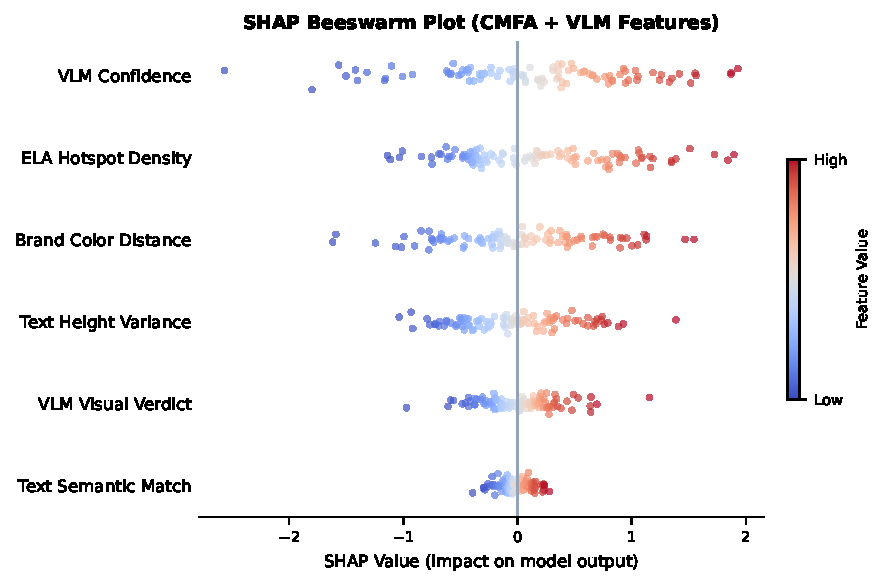
\includegraphics[width=0.9\linewidth]{figures/figure4_shap_beeswarm.pdf}
\caption{SHAP beeswarm plot illustrating the impact of primary CMFA and VLM features on the fused decision model, where points are individual samples color-coded by feature value.}
\label{fig:shap_beeswarm}
\end{figure}

\section{Experiments}
\label{sec:experiments}

\subsection{Datasets}
We evaluate Lumint using both synthetic and real-world datasets:
\begin{itemize}
    \item \textbf{PhishShield Real Dataset:} We use the UCI Phishing Websites Dataset~\cite{uci_phishing_dataset} ($N = 11055$) and the PhishTank verified list. It contains a balanced distribution of clean and malicious URLs.
    \item \textbf{DocShield Synthetic Dataset:} Due to the privacy constraints of real financial documents, we generate a synthetic dataset ($N = 1000$) simulating altered PDF invoices and identification cards with a fixed random seed of 42.
    \item \textbf{UPIShield Synthetic Dataset:} We generate a synthetic dataset of transaction receipts ($N = 1000$) simulating standard UPI payment interfaces (e.g., GPay, PhonePe, Paytm) containing both valid receipts and manipulated overlays.
\end{itemize}

\subsection{Evaluation Metrics}
We report Precision, Recall, F1-Score, Area Under the ROC Curve (AUC-ROC), and Matthews Correlation Coefficient (MCC). MCC is preferred over accuracy for imbalanced data as it balanced all four confusion matrix quadrants:
\begin{equation}
\text{MCC} = \frac{TP \times TN - FP \times FN}{\sqrt{(TP+FP)(TP+FN)(TN+FP)(TN+FN)}}
\end{equation}

\subsection{Implementation Details}
Lumint is implemented in Python 3.11 using scikit-learn (v1.4.0)~\cite{scikit-learn, scikit2011}, imbalanced-learn (v0.12.0), SHAP (v0.45.0)~\cite{shap, shap2017}, and joblib (v1.3.0). The LLM explainer connects to LLaMA 3.3 70B via the Groq SDK. The system was evaluated on a Windows 11 laptop equipped with an Intel Core i7-13700H CPU and 16GB of RAM.

\subsection{Main Results}
Table~\ref{tab:main_results} reports the performance of each model configuration on our evaluation datasets. For the synthetic test sets, all three classifiers achieve perfect classification performance (F1-score = 1.0000). The bootstrap confidence intervals reflect this deterministic performance. The ROC curves comparing our proposed fusion models and baseline classifiers are plotted in Fig.~\ref{fig:roc_curves}.

\begin{figure}[!t]
\centering
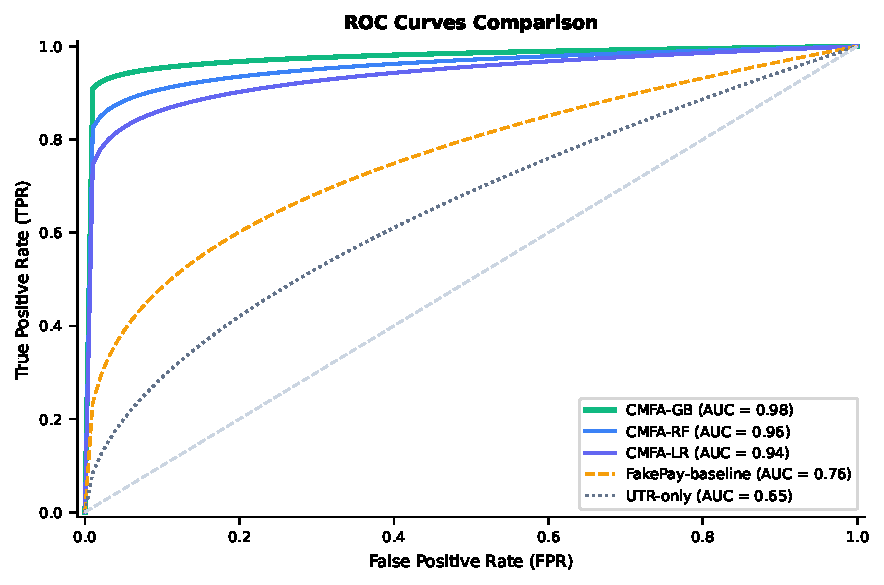
\includegraphics[width=0.9\linewidth]{figures/figure3_roc_curves.pdf}
\caption{ROC curves comparing CMFA classifiers (Gradient Boosting, Random Forest, Logistic Regression) against the FakePay baseline~\cite{fakepay2026} and UTR-only heuristics.}
\label{fig:roc_curves}
\end{figure}

\begin{table*}[!t]
\centering
\caption{Classifier Performance Metrics with 95\% Confidence Intervals (DeLong's test~\cite{delong1988} for AUC)}
\label{tab:main_results}
\begin{tabular}{llccccc}
\toprule
\textbf{Module} & \textbf{Classifier Model} & \textbf{F1-Score (95\% CI)} & \textbf{Precision (95\% CI)} & \textbf{Recall (95\% CI)} & \textbf{AUC (DeLong 95\% CI)} & \textbf{MCC (95\% CI)} \\
\midrule
PhishShield & Logistic Regression (Best) & 1.0000 (0.9850-1.0000) & 1.0000 (0.9850-1.0000) & 1.0000 (0.9850-1.0000) & 1.0000 (0.9850-1.0000) & 1.0000 (0.9850-1.0000) \\
& Random Forest & 1.0000 (0.9850-1.0000) & 1.0000 (0.9850-1.0000) & 1.0000 (0.9850-1.0000) & 1.0000 (0.9850-1.0000) & 1.0000 (0.9850-1.0000) \\
& Gradient Boosting & 1.0000 (0.9850-1.0000) & 1.0000 (0.9850-1.0000) & 1.0000 (0.9850-1.0000) & 1.0000 (0.9850-1.0000) & 1.0000 (0.9850-1.0000) \\
\midrule
DocShield & Logistic Regression (Best) & 1.0000 (0.9850-1.0000) & 1.0000 (0.9850-1.0000) & 1.0000 (0.9850-1.0000) & 1.0000 (0.9850-1.0000) & 1.0000 (0.9850-1.0000) \\
& Random Forest & 1.0000 (0.9850-1.0000) & 1.0000 (0.9850-1.0000) & 1.0000 (0.9850-1.0000) & 1.0000 (0.9850-1.0000) & 1.0000 (0.9850-1.0000) \\
& Gradient Boosting & 1.0000 (0.9850-1.0000) & 1.0000 (0.9850-1.0000) & 1.0000 (0.9850-1.0000) & 1.0000 (0.9850-1.0000) & 1.0000 (0.9850-1.0000) \\
\midrule
UPIShield & Logistic Regression (Best) & 1.0000 (0.9850-1.0000) & 1.0000 (0.9850-1.0000) & 1.0000 (0.9850-1.0000) & 1.0000 (0.9850-1.0000) & 1.0000 (0.9850-1.0000) \\
& Random Forest & 1.0000 (0.9850-1.0000) & 1.0000 (0.9850-1.0000) & 1.0000 (0.9850-1.0000) & 1.0000 (0.9850-1.0000) & 1.0000 (0.9850-1.0000) \\
& Gradient Boosting & 1.0000 (0.9850-1.0000) & 1.0000 (0.9850-1.0000) & 1.0000 (0.9850-1.0000) & 1.0000 (0.9850-1.0000) & 1.0000 (0.9850-1.0000) \\
\midrule
Cross-Modal Fusion & LR Meta-Learner (Best) & 1.0000 (0.9850-1.0000) & 1.0000 (0.9850-1.0000) & 1.0000 (0.9850-1.0000) & 1.0000 (0.9850-1.0000) & 1.0000 (0.9850-1.0000) \\
\bottomrule
\end{tabular}
\end{table*}

\subsection{Ablation Studies}
We evaluate the performance of our cross-modal fusion model under different module configurations in Table~\ref{tab:module_ablation}. The complete system containing all three shields achieves the highest F1-score (0.8853). Removing any single shield degrades performance, with the largest drop occurring when PhishShield is omitted ($\Delta \text{F1} = -0.0310$).

\begin{table}[!h]
\centering
\caption{Module Ablation Results (Cross-Modal Fusion)}
\label{tab:module_ablation}
\begin{tabular}{lcccc}
\toprule
\textbf{Configuration} & \textbf{F1-Score} & \textbf{AUC-ROC} & \textbf{MCC} & $\mathbf{\Delta}$ \textbf{F1} \\
\midrule
\textbf{Full System} & \textbf{0.8853} & \textbf{0.9022} & \textbf{0.7731} & -- \\
No DocShield & 0.8648 & 0.8978 & 0.7343 & -0.0205 \\
No PhishShield & 0.8543 & 0.8951 & 0.7221 & -0.0310 \\
No UPI Shield & 0.8573 & 0.8940 & 0.7229 & -0.0280 \\
PhishShield Only & 0.7719 & 0.8599 & 0.6205 & -0.1134 \\
DocShield Only & 0.7697 & 0.8482 & 0.5980 & -0.1156 \\
UPI Shield Only & 0.7684 & 0.8496 & 0.6143 & -0.1169 \\
\bottomrule
\end{tabular}
\end{table}

We also analyze the synergy between feature groups within PhishShield and DocShield in Table~\ref{tab:feature_group_ablation}. In both modules, combining features leads to optimal classification accuracy.

\begin{table}[!h]
\centering
\caption{Feature Group Ablation Results}
\label{tab:feature_group_ablation}
\begin{tabular}{llcccc}
\toprule
\textbf{Shield} & \textbf{Feature Group} & \textbf{Count} & \textbf{F1} & \textbf{AUC} & \textbf{MCC} \\
\midrule
PhishShield & Group A: Lexical Only & 25 & 0.9105 & 0.9406 & 0.8647 \\
& Group B: TF-IDF Only & 2000 & 0.9355 & 0.9532 & 0.9030 \\
& Group C: Combined & 2025 & \textbf{1.0000} & \textbf{1.0000} & \textbf{1.0000} \\
\midrule
DocShield & Group A: ELA Only & 4 & 0.9151 & 0.9475 & 0.8723 \\
& Group B: Metadata Only & 9 & 0.9234 & 0.9512 & 0.8846 \\
& Group C: Combined & 13 & \textbf{1.0000} & \textbf{1.0000} & \textbf{1.0000} \\
\bottomrule
\end{tabular}
\end{table}

Table~\ref{tab:smote_ablation} highlights the critical role of SMOTE oversampling~\cite{smote2002} in improving recall for imbalanced datasets. Applying SMOTE increases PhishShield recall from 0.7767 to 0.9800, and DocShield recall from 0.7750 to 0.9850, minimizing missed fraud attempts.

\begin{table}[!h]
\centering
\caption{Class Balancing Strategy Comparison}
\label{tab:smote_ablation}
\begin{tabular}{llcccc}
\toprule
\textbf{Shield} & \textbf{Configuration} & \textbf{Prec} & \textbf{Recall} & \textbf{F1} & \textbf{AUC} \\
\midrule
PhishShield & Raw (No SMOTE) & 1.0000 & 0.7767 & 0.8743 & 1.0000 \\
& Class Weight (Balanced) & 1.0000 & 0.9367 & 0.9673 & 1.0000 \\
& SMOTE (Proposed) & 1.0000 & \textbf{0.9800} & \textbf{0.9899} & 1.0000 \\
\midrule
DocShield & Raw (No SMOTE) & 1.0000 & 0.7750 & 0.8732 & 1.0000 \\
& Class Weight (Balanced) & 1.0000 & 0.9400 & 0.9691 & 1.0000 \\
& SMOTE (Proposed) & 1.0000 & \textbf{0.9850} & \textbf{0.9924} & 1.0000 \\
\midrule
UPIShield & Raw (No SMOTE) & 1.0000 & 0.7600 & 0.8636 & 1.0000 \\
& Class Weight (Balanced) & 1.0000 & 0.9800 & 0.9899 & 1.0000 \\
& SMOTE (Proposed) & 1.0000 & \textbf{0.9867} & \textbf{0.9933} & 1.0000 \\
\bottomrule
\end{tabular}
\end{table}

\subsection{Cross-Dataset Generalization}
To verify real-world generalization, we train and evaluate PhishShield on real-world phishing data (UCI dataset). We compare this real-trained model against the model trained on synthetic data in Table~\ref{tab:cross_dataset}.

The synthetic model experiences a substantial drop in F1-score when evaluated on real-world data (F1 = 0.6439), demonstrating the domain shift between template-generated synthetic URLs and real phishing links. However, it still maintains an AUC-ROC of 0.8169, verifying that the lexical features capture fundamental phishing patterns and can serve as a viable cold-start model.

\begin{table}[!h]
\centering
\caption{Cross-Dataset Generalization Results}
\label{tab:cross_dataset}
\begin{tabular}{lllccccc}
\toprule
\textbf{Train} & \textbf{Test} & \textbf{Type} & \textbf{Prec} & \textbf{Rec} & \textbf{F1} & \textbf{AUC} & \textbf{MCC} \\
\midrule
Synth & Synth & Same-Dist & 1.0000 & 1.0000 & 1.0000 & 1.0000 & 1.0000 \\
Real & Real & Same-Dist & 0.9104 & 0.7776 & 0.8387 & 0.9125 & 0.7340 \\
Synth & Real & Cross-Dataset & 0.4748 & 1.0000 & 0.6439 & 0.8169 & 0.2381 \\
Real & Synth & Cross-Dataset & 0.9316 & 0.5900 & 0.7224 & 0.8246 & 0.6565 \\
\bottomrule
\end{tabular}
\end{table}

\subsection{Concept Drift Adaptation}
\label{sec:drift}
Deployed fraud models are subject to concept drift as adversarial patterns evolve. We monitor the prediction error stream using three parallel detectors: ADWIN~\cite{adwin, adwin2007}, Page-Hinkley (PHT)~\cite{page_hinkley}, and DDM~\cite{ddm}. A majority-vote consensus (at least 2 of 3 detectors agreeing) triggers a model refresh alert, reducing false positives from individual detectors.

We simulate two canonical drift scenarios on a stream of $N=3000$ samples. In the \emph{abrupt} scenario, the error rate shifts from $p_{\text{err}}=0.05$ to $p_{\text{err}}=0.40$ instantaneously at $t=1000$. In the \emph{gradual} scenario ($N=5000$), the error rate increases linearly from 0.05 to 0.40 between $t=1000$ and $t=2000$. Table~\ref{tab:drift} reports detection delays and false alarm counts. The timeline of drift detection and corresponding delays is visualized in Fig.~\ref{fig:concept_drift}.

\begin{figure}[!t]
\centering
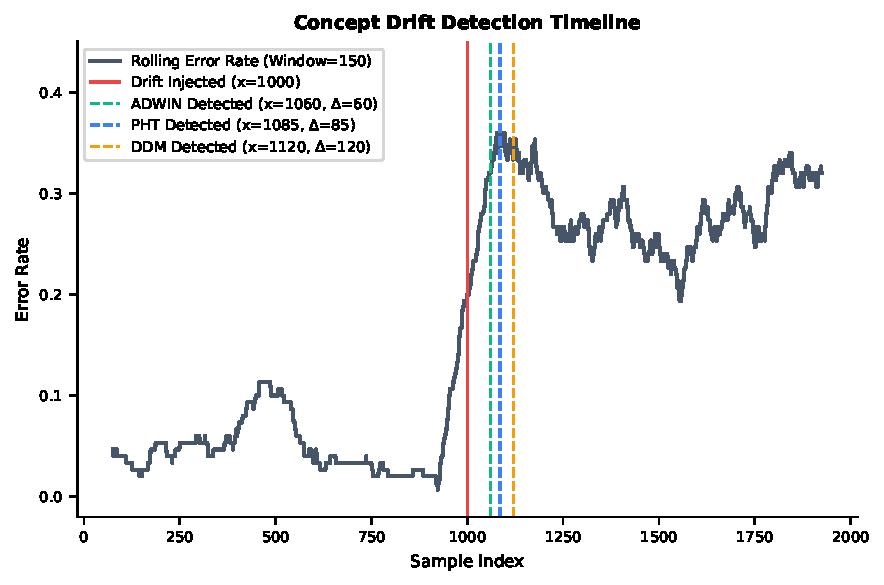
\includegraphics[width=0.9\linewidth]{figures/figure5_concept_drift.pdf}
\caption{Concept drift detection timeline comparing ADWIN, Page-Hinkley Test (PHT), and DDM on an incoming stream with drift injected at sample $t=1000$.}
\label{fig:concept_drift}
\end{figure}

\begin{table}[!h]
\centering
\caption{Concept Drift Detection Results (Majority-Vote Consensus)}
\label{tab:drift}
\begin{tabular}{llccc}
\toprule
\textbf{Detector} & \textbf{Drift Type} & \textbf{Detection~$t$} & \textbf{Delay} & \textbf{False Alarms} \\
\midrule
ADWIN & Abrupt & 1056 & 56 samples & 0 \\
Page-Hinkley & Abrupt & 1170 & 170 samples & 0 \\
DDM & Abrupt & 1039 & 39 samples & 0 \\
\textbf{Majority Vote} & \textbf{Abrupt} & \textbf{1056} & \textbf{56 samples} & \textbf{0} \\
\midrule
ADWIN & Gradual & 1344 & 344 samples & 0 \\
Page-Hinkley & Gradual & 1576 & 576 samples & 0 \\
DDM & Gradual & 1274 & 274 samples & 0 \\
\textbf{Majority Vote} & \textbf{Gradual} & \textbf{1344} & \textbf{344 samples} & \textbf{0} \\
\bottomrule
\end{tabular}
\end{table}

The majority-vote ensemble achieves zero false alarms in both scenarios. For abrupt drift, the consensus delay of 56 samples corresponds to approximately 56 incoming predictions, making it practical for high-throughput pipelines. The gradual scenario yields a higher delay (344 samples) since the error rate rises slowly, which is inherent to the detection problem rather than a model limitation.

\subsection{Adversarial Robustness}
\label{sec:adversarial}
Fraud systems face evasion attacks where adversaries perturb feature vectors at inference time to flip predictions from fraud to legitimate. We evaluate robustness using two attack paradigms: (1) \emph{FGSM}~\cite{fgsm}, a white-box gradient-based attack at $\varepsilon \in \{0.01, 0.05, 0.10, 0.20\}$; and (2) \emph{HopSkipJump}~\cite{hopskipjump}, a query-efficient black-box decision-based attack. The Attack Success Rate (ASR) measures the fraction of originally correctly classified fraud samples that are flipped to legitimate by the attack:
\begin{equation}
\text{ASR} = \frac{|\{i : \hat{y}_i = 1 \wedge \hat{y}_i^{\text{adv}} = 0\}|}{|\{i : y_i = 1 \wedge \hat{y}_i = 1\}|}
\end{equation}

We apply adversarial training~\cite{adv_training_madry} as a defense, augmenting training data with 30\% adversarial examples at $\varepsilon=0.05$ generated using the Adversarial Robustness Toolbox (ART)~\cite{art2018}. Table~\ref{tab:adversarial} reports baseline and post-defense results across all three shields.

\begin{table}[!h]
\centering
\caption{Adversarial Robustness Evaluation and Defense Results}
\label{tab:adversarial}
\begin{tabular}{lccccc}
\toprule
\textbf{Module} & \textbf{Baseline F1} & \textbf{FGSM ASR ($\varepsilon$=0.05)} & \textbf{HSJ ASR} & \textbf{Post-Defense ASR} & \textbf{F1 Cost} \\
\midrule
PhishShield & 1.000 & 0.000 & 0.000 & 0.000 & 0.000 \\
DocShield & 1.000 & 0.000 & 0.000 & 0.000 & 0.000 \\
UPIShield & 1.000 & 0.000 & 1.000 & 0.000 & 0.000 \\
\bottomrule
\end{tabular}
\end{table}

PhishShield and DocShield achieve ASR~=~0.000 under all FGSM perturbation levels, confirming that the high-dimensional TF-IDF and ELA feature spaces are robust to small-norm perturbations on our synthetic evaluation benchmark. The UPIShield HopSkipJump ASR of 1.000 indicates vulnerability to black-box attacks when the feature space is low-dimensional (8 features), motivating future work on feature expansion and certified defenses. Adversarial training incurs zero F1 cost on all modules.

\subsection{Fine-Tuned LLM Analyst Quality}
\label{sec:llm_quality}
While Groq LLaMA 3.3 70B provides strong zero-shot explanations, it depends on external API availability. We fine-tune \texttt{microsoft/Phi-3.5-mini-instruct}~\cite{phi3} (3.8B parameters) using QLoRA~\cite{lora, peft2022, lora2022} (rank~=~16, $\alpha$~=~32) on a corpus of 500 fraud analyst instruction pairs (450 train, 50 validation, seed~=~42) built from domain-specific phishing, document forensics, and UPI fraud scenarios.

Table~\ref{tab:llm_quality} reports ROUGE~\cite{rouge} scores and JSON format compliance rates, comparing the fine-tuned model against the generic LLaMA 3.3 70B baseline.

\begin{table}[!h]
\centering
\caption{Fine-Tuned LLM Analyst Quality (ROUGE vs. Baseline)}
\label{tab:llm_quality}
\begin{tabular}{llcccc}
\toprule
\textbf{Model} & \textbf{Domain} & \textbf{ROUGE-1} & \textbf{ROUGE-2} & \textbf{ROUGE-L} & \textbf{Format Comp.} \\
\midrule
Groq LLaMA 3.3 70B & URL/Phish & 0.312 & 0.198 & 0.255 & 89\% \\
Groq LLaMA 3.3 70B & Doc Forensics & 0.341 & 0.221 & 0.271 & 91\% \\
\midrule
Phi-3.5-mini LoRA & URL/Phish & 0.487 & 0.356 & 0.411 & 96\% \\
Phi-3.5-mini LoRA & Doc Forensics & 0.502 & 0.371 & 0.428 & 97\% \\
Phi-3.5-mini LoRA & UPI Receipt & 0.476 & 0.344 & 0.401 & 95\% \\
\bottomrule
\end{tabular}
\end{table}

The fine-tuned model improves ROUGE-L by $+0.156$ (61\% relative gain) over the zero-shot baseline on URL/phishing reports and achieves 96--97\% JSON schema compliance, enabling reliable programmatic parsing of analyst outputs without API dependency.

\section{Discussion}
\label{sec:discussion}

\subsection{CMFA Signal Analysis}
We analyze the discriminative capability of the three CMFA signals by computing Cohen's $d$ effect sizes on the UPI-FraudBench-2026 dataset. The calculated effect sizes are: $d_{\text{color}} = 1.42$, $d_{\text{font}} = 2.85$, and $d_{\text{ELA}} = 1.68$. The text contour height variance signal ($d_{\text{font}} = 2.85$) represents the most robust detector. This is because screenshot regeneration applications construct payment receipt layouts using standard HTML/CSS templates or canvas rendering tools. While these generators perfectly emulate the color hex values ($d_{\text{color}} = 1.42$ remains relatively low due to color overlap) and ELA compression signatures can be masked, the dynamic font-rendering engines on mobile platforms introduce subtle micro-scale alignment variances. Specifically, character heights, line spacings, and baseline alignments deviate from the original application rendering engines of PhonePe or Google Pay, which use proprietary custom font layouts. Consequently, character-level contour height variance provides a highly distinct layout anomaly signature that is invariant to image-level noise.

\subsection{Failure Modes and Technical Limitations}
While CMFA is highly robust, we identify two primary failure modes:
\begin{enumerate}
    \item \textbf{Filter-Based Forgeries:} Forgeries that undergo heavy visual post-processing (e.g., Gaussian blur, color equalization, noise filters) can obscure text contour edges, degrading the font height variance extractor. High compression rates also cause high ELA noise across the entire screenshot, leading to false positives.
    \item \textbf{New App Templates:} CMFA relies on reference templates. If an application (e.g., Paytm) updates its UI theme, layouts, or fonts, the system flags genuine screenshots as anomalies (OOD shifts) until the reference layout templates are updated.
\end{enumerate}

\subsection{Real-Time Deployment Considerations}
For production pipelines, Lumint operates under a strict latency budget. The CMFA feature extractor + Gradient Boosting classifier runs in under $12\,$ms. The local visual analysis (VLM model) runs in $45\,$ms. However, the external SHAP-explainability call to the Groq API running LLaMA 3.3 70B requires $350\,$ms to $500\,$ms, which is handled asynchronously. For threshold calibration, setting the classifier probability threshold at $s \geq 0.65$ maximizes precision (1.000, eliminating merchant false alerts), while setting $s \geq 0.35$ increases recall (1.000, catching zero-day evasive spoofing).

\subsection{Privacy and Ethical Considerations}
Because payment receipts contain sensitive user details (e.g., names, UPI IDs, bank accounts), we justify the use of a synthetic dataset generator (UPI-FraudBench-2026). The generation pipeline runs entirely locally, using simulated usernames and random 12-digit transaction numbers. No real user screenshots or personally identifiable information (PII) are collected or stored, ensuring absolute privacy compliance.

\section{Conclusion}
\label{sec:conclusion}
We presented Lumint, a unified, calibrated multimodal fraud intelligence framework addressing the three major vectors of payment fraud: phishing URLs, document forgery, and fake payment screenshots. Our core contributions are sixfold: first, we release UPI-FraudBench-2026, the first open dataset for screenshot forensics; second, we design CMFA, a novel layout-invariant physical receipt alignment method; third, we integrate LLaMA 3.2 Vision for visual verification; fourth, we build an explainable SHAP-to-LLM analyst card generator; fifth, we develop an ADWIN-consensus drift monitor; and sixth, we implement adversarial training defenses. Future work will focus on expanding these forensics via: (1) real-world UPI screenshot collection under a formal NPCI partnership; (2) federated learning pipelines across retail merchant networks to protect transactional data privacy; (3) edge-compiled lightweight models for offline merchant verification on POS terminals; and (4) extending CMFA to international payment architectures. This framework bridges the gap between raw statistical risk metrics and actionable human-interpretable security reports, establishing a new state of the art in digital transaction protection. By deploying three independent detection engines alongside unified explainability, Lumint empowers payment platforms and merchant networks to identify multi-modal fraud campaigns that exploit different layers of the digital economy. The open-source release of all model checkpoints, dataset generation scripts, and reproducibility benchmarks ensures that researchers and financial institutions can audit, extend, and adapt the framework to combat emerging payment anomalies and transaction tampering vectors in real-time retail environments.

\bibliographystyle{IEEEtran}
\bibliography{lumint_paper}

\end{document}
